%% Modified for NDSS 2015 on 2014/08/07

\documentclass[conference]{IEEEtran}

\pagestyle{plain}


% *** CITATION PACKAGES ***
%
%\usepackage{cite}
% cite.sty was written by Donald Arseneau
% V1.6 and later of IEEEtran pre-defines the format of the cite.sty package
% \cite{} output to follow that of IEEE. Loading the cite package will
% result in citation numbers being automatically sorted and properly
% "compressed/ranged". e.g., [1], [9], [2], [7], [5], [6] without using
% cite.sty will become [1], [2], [5]--[7], [9] using cite.sty. cite.sty's
% \cite will automatically add leading space, if needed. Use cite.sty's
% noadjust option (cite.sty V3.8 and later) if you want to turn this off.
% cite.sty is already installed on most LaTeX systems. Be sure and use
% version 4.0 (2003-05-27) and later if using hyperref.sty. cite.sty does
% not currently provide for hyperlinked citations.
% The latest version can be obtained at:
% http://www.ctan.org/tex-archive/macros/latex/contrib/cite/
% The documentation is contained in the cite.sty file itself.

% ----------------------------------------------------------------------------------------

% *** GRAPHICS RELATED PACKAGES ***
%
\ifCLASSINFOpdf
  % \usepackage[pdftex]{graphicx}
  % declare the path(s) where your graphic files are
  % \graphicspath{{../pdf/}{../jpeg/}}
  % and their extensions so you won't have to specify these with
  % every instance of \includegraphics
  % \DeclareGraphicsExtensions{.pdf,.jpeg,.png}
\else
  % or other class option (dvipsone, dvipdf, if not using dvips). graphicx
  % will default to the driver specified in the system graphics.cfg if no
  % driver is specified.
  % \usepackage[dvips]{graphicx}
  % declare the path(s) where your graphic files are
  % \graphicspath{{../eps/}}
  % and their extensions so you won't have to specify these with
  % every instance of \includegraphics
  % \DeclareGraphicsExtensions{.eps}
\fi
% graphicx was written by David Carlisle and Sebastian Rahtz. It is
% required if you want graphics, photos, etc. graphicx.sty is already
% installed on most LaTeX systems. The latest version and documentation can
% be obtained at: 
% http://www.ctan.org/tex-archive/macros/latex/required/graphics/
% Another good source of documentation is "Using Imported Graphics in
% LaTeX2e" by Keith Reckdahl which can be found as epslatex.ps or
% epslatex.pdf at: http://www.ctan.org/tex-archive/info/
%
% latex, and pdflatex in dvi mode, support graphics in encapsulated
% postscript (.eps) format. pdflatex in pdf mode supports graphics
% in .pdf, .jpeg, .png and .mps (metapost) formats. Users should ensure
% that all non-photo figures use a vector format (.eps, .pdf, .mps) and
% not a bitmapped formats (.jpeg, .png). IEEE frowns on bitmapped formats
% which can result in "jaggedy"/blurry rendering of lines and letters as
% well as large increases in file sizes.
%
% You can find documentation about the pdfTeX application at:
% http://www.tug.org/applications/pdftex

% ----------------------------------------------------------------------------------------

% *** MATH PACKAGES ***
%
%\usepackage[cmex10]{amsmath}
% A popular package from the American Mathematical Society that provides
% many useful and powerful commands for dealing with mathematics. If using
% it, be sure to load this package with the cmex10 option to ensure that
% only type 1 fonts will utilized at all point sizes. Without this option,
% it is possible that some math symbols, particularly those within
% footnotes, will be rendered in bitmap form which will result in a
% document that can not be IEEE Xplore compliant!
%
% Also, note that the amsmath package sets \interdisplaylinepenalty to 10000
% thus preventing page breaks from occurring within multiline equations. Use:
%\interdisplaylinepenalty=2500
% after loading amsmath to restore such page breaks as IEEEtran.cls normally
% does. amsmath.sty is already installed on most LaTeX systems. The latest
% version and documentation can be obtained at:
% http://www.ctan.org/tex-archive/macros/latex/required/amslatex/math/

% ----------------------------------------------------------------------------------------

% *** SPECIALIZED LIST PACKAGES ***
%
%\usepackage{algorithmic}
% algorithmic.sty was written by Peter Williams and Rogerio Brito.
% This package provides an algorithmic environment fo describing algorithms.
% You can use the algorithmic environment in-text or within a figure
% environment to provide for a floating algorithm. Do NOT use the algorithm
% floating environment provided by algorithm.sty (by the same authors) or
% algorithm2e.sty (by Christophe Fiorio) as IEEE does not use dedicated
% algorithm float types and packages that provide these will not provide
% correct IEEE style captions. The latest version and documentation of
% algorithmic.sty can be obtained at:
% http://www.ctan.org/tex-archive/macros/latex/contrib/algorithms/
% There is also a support site at:
% http://algorithms.berlios.de/index.html
% Also of interest may be the (relatively newer and more customizable)
% algorithmicx.sty package by Szasz Janos:
% http://www.ctan.org/tex-archive/macros/latex/contrib/algorithmicx/

% ----------------------------------------------------------------------------------------

% *** ALIGNMENT PACKAGES ***
%
%\usepackage{array}
% Frank Mittelbach's and David Carlisle's array.sty patches and improves
% the standard LaTeX2e array and tabular environments to provide better
% appearance and additional user controls. As the default LaTeX2e table
% generation code is lacking to the point of almost being broken with
% respect to the quality of the end results, all users are strongly
% advised to use an enhanced (at the very least that provided by array.sty)
% set of table tools. array.sty is already installed on most systems. The
% latest version and documentation can be obtained at:
% http://www.ctan.org/tex-archive/macros/latex/required/tools/


%\usepackage{mdwmath}
%\usepackage{mdwtab}
% Also highly recommended is Mark Wooding's extremely powerful MDW tools,
% especially mdwmath.sty and mdwtab.sty which are used to format equations
% and tables, respectively. The MDWtools set is already installed on most
% LaTeX systems. The lastest version and documentation is available at:
% http://www.ctan.org/tex-archive/macros/latex/contrib/mdwtools/

% IEEEtran contains the IEEEeqnarray family of commands that can be used to
% generate multiline equations as well as matrices, tables, etc., of high
% quality.


%\usepackage{eqparbox}
% Also of notable interest is Scott Pakin's eqparbox package for creating
% (automatically sized) equal width boxes - aka "natural width parboxes".
% Available at:
% http://www.ctan.org/tex-archive/macros/latex/contrib/eqparbox/


% *** SUBFIGURE PACKAGES ***
%\usepackage[tight,footnotesize]{subfigure}
% subfigure.sty was written by Steven Douglas Cochran. This package makes it
% easy to put subfigures in your figures. e.g., "Figure 1a and 1b". For IEEE
% work, it is a good idea to load it with the tight package option to reduce
% the amount of white space around the subfigures. subfigure.sty is already
% installed on most LaTeX systems. The latest version and documentation can
% be obtained at:
% http://www.ctan.org/tex-archive/obsolete/macros/latex/contrib/subfigure/
% subfigure.sty has been superceeded by subfig.sty.


%\usepackage[caption=false]{caption}
%\usepackage[font=footnotesize]{subfig}
% subfig.sty, also written by Steven Douglas Cochran, is the modern
% replacement for subfigure.sty. However, subfig.sty requires and
% automatically loads Axel Sommerfeldt's caption.sty which will override
% IEEEtran.cls handling of captions and this will result in nonIEEE style
% figure/table captions. To prevent this problem, be sure and preload
% caption.sty with its "caption=false" package option. This is will preserve
% IEEEtran.cls handing of captions. Version 1.3 (2005/06/28) and later 
% (recommended due to many improvements over 1.2) of subfig.sty supports
% the caption=false option directly:
%\usepackage[caption=false,font=footnotesize]{subfig}
%
% The latest version and documentation can be obtained at:
% http://www.ctan.org/tex-archive/macros/latex/contrib/subfig/
% The latest version and documentation of caption.sty can be obtained at:
% http://www.ctan.org/tex-archive/macros/latex/contrib/caption/


% *** FLOAT PACKAGES ***
%
%\usepackage{fixltx2e}
% fixltx2e, the successor to the earlier fix2col.sty, was written by
% Frank Mittelbach and David Carlisle. This package corrects a few problems
% in the LaTeX2e kernel, the most notable of which is that in current
% LaTeX2e releases, the ordering of single and double column floats is not
% guaranteed to be preserved. Thus, an unpatched LaTeX2e can allow a
% single column figure to be placed prior to an earlier double column
% figure. The latest version and documentation can be found at:
% http://www.ctan.org/tex-archive/macros/latex/base/


%\usepackage{stfloats}
% stfloats.sty was written by Sigitas Tolusis. This package gives LaTeX2e
% the ability to do double column floats at the bottom of the page as well
% as the top. (e.g., "\begin{figure*}[!b]" is not normally possible in
% LaTeX2e). It also provides a command:
%\fnbelowfloat
% to enable the placement of footnotes below bottom floats (the standard
% LaTeX2e kernel puts them above bottom floats). This is an invasive package
% which rewrites many portions of the LaTeX2e float routines. It may not work
% with other packages that modify the LaTeX2e float routines. The latest
% version and documentation can be obtained at:
% http://www.ctan.org/tex-archive/macros/latex/contrib/sttools/
% Documentation is contained in the stfloats.sty comments as well as in the
% presfull.pdf file. Do not use the stfloats baselinefloat ability as IEEE
% does not allow \baselineskip to stretch. Authors submitting work to the
% IEEE should note that IEEE rarely uses double column equations and
% that authors should try to avoid such use. Do not be tempted to use the
% cuted.sty or midfloat.sty packages (also by Sigitas Tolusis) as IEEE does
% not format its papers in such ways.


% *** PDF, URL AND HYPERLINK PACKAGES ***
%
%\usepackage{url}
% url.sty was written by Donald Arseneau. It provides better support for
% handling and breaking URLs. url.sty is already installed on most LaTeX
% systems. The latest version can be obtained at:
% http://www.ctan.org/tex-archive/macros/latex/contrib/misc/
% Read the url.sty source comments for usage information. Basically,
% \url{my_url_here}.

% ----------------------------------------------------------------------------------------

\usepackage{mathtools}
\usepackage[urlbordercolor={1 1 1},citebordercolor={1 1 1},linkbordercolor={1 1 1}]{hyperref}
%\usepackage{enumitem}
\usepackage{tikz}
\usetikzlibrary{decorations.text}
\usepackage{tkz-berge}
\usepackage{amsmath}
\usepackage{tabularx}

% https://tex.stackexchange.com/questions/42271/floor-and-ceiling-functions
\DeclarePairedDelimiter{\ceil}{\lceil}{\rceil}
\DeclarePairedDelimiter{\floor}{\lfloor}{\rfloor}

\newcommand*\concat{\mathbin{\|}}

% *** Do not adjust lengths that control margins, column widths, etc. ***
% *** Do not use packages that alter fonts (such as pslatex).         ***
% There should be no need to do such things with IEEEtran.cls V1.6 and later.
% (Unless specifically asked to do so by the journal or conference you plan
% to submit to, of course. )

\begin{document}

\title{The Onion Name System: \\ \huge Tor-powered Distributed DNS for Tor Hidden Services}

% author names and affiliations
% use a multiple column layout for up to three different
% affiliations
\author{
	\IEEEauthorblockN{[Anonymous submission]}
	\IEEEauthorblockA{}
}
	
%	\IEEEauthorblockN{Jesse Victors}
%	\IEEEauthorblockA{Utah State University \\ jvictors@jessevictors.com}
%	\and
%	\IEEEauthorblockN{Ming Li}
%	\IEEEauthorblockA{University of Arizona \\ lim@email.arizona.edu}
%	\and
%	\IEEEauthorblockN{Xinwen Fu}
%	\IEEEauthorblockA{University of Massachusetts Lowell \\ xinwenfu@cs.uml.edu}

\IEEEoverridecommandlockouts
\makeatletter\def\@IEEEpubidpullup{9\baselineskip}\makeatother
\IEEEpubid{\parbox{\columnwidth}{Permission to freely reproduce all or part
    of this paper for noncommercial purposes is granted provided that
    copies bear this notice and the full citation on the first
    page. Reproduction for commercial purposes is strictly prohibited
    without the prior written consent of the Internet Society, the
    first-named author (for reproduction of an entire paper only), and
    the author's employer if the paper was prepared within the scope
    of employment.  \\
    NDSS '15, 8-11 February 2015, San Diego, CA, USA\\
    Copyright 2015 Internet Society, ISBN <TBD>\\
    http://dx.doi.org/10.14722/ndss.2015.23xxx
}
\hspace{\columnsep}\makebox[\columnwidth]{}}


% make the title area
\maketitle

\begin{abstract}

Tor hidden services are anonymous servers of unknown location and ownership who can be accessed through any Tor-enabled web browser. They have gained popularity over the years, but still suffer from major usability challenges due to their cryptographically-generated non-memorable addresses.

In response to this difficulty, in this work we introduce the Onion Name System (OnioNS), a privacy-enhanced distributed DNS that allows users to reference a hidden service by a meaningful globally-unique verifiable domain name chosen by the hidden service operator. We introduce a new distributed self-healing public ledger and construct OnioNS as an optional backwards-compatible plugin for Tor on top of existing hidden service infrastructure. We simplify our design and threat model by embedding OnioNS within the Tor network and provide mechanisms for authenticated denial-of-existence with minimal networking costs. Our reference implementation demonstrates that OnioNS successfully addresses the major usability issue that has been with Tor hidden services since their introduction in 2002.

\end{abstract}

% IEEEtran.cls defaults to using nonbold math in the Abstract.
% This preserves the distinction between vectors and scalars. However,
% if the conference you are submitting to favors bold math in the abstract,
% then you can use LaTeX's standard command \boldmath at the very start
% of the abstract to achieve this. Many IEEE journals/conferences frown on
% math in the abstract anyway.

% no keywords

% For peer review papers, you can put extra information on the cover
% page as needed:
% \ifCLASSOPTIONpeerreview
% \begin{center} \bfseries EDICS Category: 3-BBND \end{center}
% \fi
%
% For peerreview papers, this IEEEtran command inserts a page break and
% creates the second title. It will be ignored for other modes.
%%\IEEEpeerreviewmaketitle

\section{Introduction}

As the prevalence of the Internet and other communication has grown, so too has the development and usage of privacy-enhancing systems. These are protocols that provide privacy by obfuscating the link between a user's identity or location and their communications. Following a general distrust of unsecured Internet communications and in light of the 2013-current revelations by Edward Snowden of international Internet mass-surveillance, users have increasingly turned to these tools for their own protection.

Tor\cite{dingledine2004tor} is a third-generation onion routing system and is the most popular low-latency anonymous communication network in use today. In Tor, users construct a layered encrypted communications circuit over three onion routers in order to mask their identity and location. As messages travel through the circuit, each onion router in turn decrypts their encryption layer, exposing their respective routing information. This provides end-to-end communication confidentiality of the sender.

Tor users interact with the Internet and other systems over Tor via the Tor Browser, a security-enhanced fork of Firefox ESR. This achieves a level of usability but also security: Tor achieves most of its application-level sanitization via privacy filters in the Tor Browser; unlike its predecessors, Tor performs little sanitization itself. Tor's threat model assumes that the capabilities of adversaries are limited to traffic analysis attacks on a restricted scale; they may observe or manipulate portions of Tor traffic, that they may run onion routers themselves, and that they may compromise a fraction of other existing routers. Tor's design centers around usability and defense against these types of attacks.

\subsection{Motivation}

Tor also supports \emph{hidden services} -- anonymous servers that intentionally mask their IP address through Tor circuits. They utilize the .onion pseudo-TLD, preventing hidden services from being accessed outside the context of Tor. Hidden services are only known by their public RSA key and typically referenced by their address, 16 base32-encoded characters derived from the SHA-1 hash of the server's key. This builds a publicly-confirmable one-to-one relationship between the public key and its address and allows hidden services to be accessed via the Tor Browser by their address within a distributed environment.

\begin{figure}[htbp]
	\centering
	\includegraphics[width=0.9\linewidth]{../assets/images/LucidCharts/Hidden_Services.pdf}
	\caption{A Tor client, Alice, and a hidden service, Bob, first mate two Tor circuits (purple and red) at one of Bob's long-term \emph{introduction points} (IP). They then renegotiate and communicate over another pair of Tor circuits (blue and green) at an ephemeral \emph{rendezvous point} (RP). This achieves communication with bi-directional anonymity\cite{overlier2006locating}.}
\end{figure}

Tor hidden service addresses are distributed and globally collision-free, but there is a strong discontinuity between the address and the service's purpose. For example, a visitor cannot determine that \url{3g2upl4pq6kufc4m.onion} is the DuckDuckGo search engine without visiting the hidden service. Generally speaking, it is currently impossible to categorize or fully label hidden services in advance. Over time, third-party directories -- both on the Clearnet and Darknet -- have appeared in attempt to counteract this issue, but these directories must be constantly maintained and the approach is neither convenient nor does it scale well. Given the approximately 27,000 hidden services on the Tor network,  (Figure \ref{fig:OnionCount}) this suggests the strong need for a more complete solution to solve the usability issue.

\begin{figure}[htbp]
	\centering
	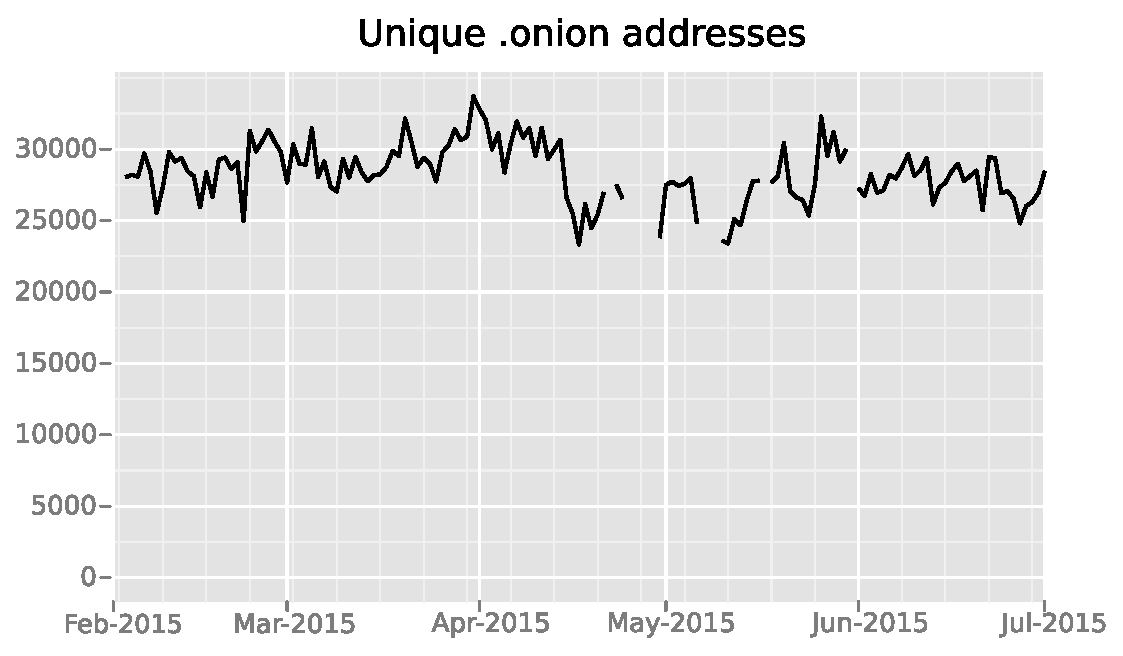
\includegraphics[width=\linewidth]{../assets/images/Tor/onion_2015-02_2015-07.eps}
	\caption{The number of unique .onion addresses seen in the Tor network between February 2015 and July 2015\cite{kadianakis2015extrapolating}\cite{TorMetrics}.}
	\label{fig:OnionCount}
\end{figure}

\subsection{Contributions}

In this paper, we present the design, analysis and implementation of the Onion Name System, (OnioNS) a distributed, secure, and usable domain name system for Tor hidden services. Any hidden service can anonymously register an association between a meaningful human-readable domain name and a target hidden service and clients can query against OnioNS in a privacy-preserving and verifiable manner. OnioNS is powered by a random subset of nodes within the existing infrastructure of Tor, significantly limiting the additional attack surface. We devise a distributed DNS database using a blockchain-based data structure that is tamper-proof, self-healing, resistant to node compromise, and provides authenticated denial-of-existence. We design OnioNS as a backwards-compatible plugin to the Tor software. Our prototype implementation demonstrates the high usability and performance of OnioNS. To the best of our knowledge, this is the first alternative DNS for Tor hidden services which is distributed, secure, and usable at the same time.

\textbf{Paper Organization:} This paper is divided into four main sections. In section \ref{sec:problemStatement} we define our design objectives and explain why existing works do not meet our goals. We also define our threat model, which closely matches Tor's model with one additional assumption. In section \ref{sec:Solution}, we describe the system overview and define several key protocols. In section \ref{sec:Analysis} we analyse the security of our assumptions and examine other attack vectors. Last, in section \ref{sec:Analysis} we evaluate our implementation prototype and show that it can access a hidden service under a meaningful domain name.

\section{Problem Statement}
\label{sec:problemStatement}

To integrate with Tor, we must provide a secure system, preserve user privacy, and avoid compromising other areas of the Tor network. Additionally, we seek to achieve all three properties of Zooko's Triangle (section \ref{sec:ZookosTriangle}) and to providing a mechanism for authenticated denial-of-existence (section \ref{sec:authDenialIntro}).

\subsection{Design Objectives}

Here we enumerate a list of requirements that must be met by any DNS applicable to Tor hidden services. In Section \ref{sec:RelatedWorks} we analyse existing works and show how these systems do not meet these requirements and in Section \ref{sec:Solution} we demonstrate how we overcome them with OnioNS.

1. \textbf{The system must support anonymous registrations.} The system should not require any personally-identifiable or location information from the registrant. Tor hidden services publicize no more information than a public key and Introduction Points.

2. \textbf{The system must support privacy-enhanced queries.} Clients should be anonymous, indistinguishable, and unable to be tracked by name servers.

3. \textbf{Registrations must be authenticable.} Clients must be able to verify that the domain-address pairing that they receive from name servers is authentic relative to the authenticity of the hidden service.

4. \textbf{Domain names must be globally unique.} Any domain name of global scope must point to at most one server. For naming systems that generate names via cryptographic hashes, the key-space must be of sufficient length to resist cryptanalytic attack.

5. \textbf{The system must be distributed.} Systems with root authorities have distinct disadvantages compared to distributed networks: specifically, central authorities have absolute control over the system and root security breaches could easily compromise the integrity of the entire system. Root authorities may also be able to compromise the privacy of both users and hidden services or may not allow anonymous registrations.

6. \textbf{The system must be relatively easy to use.} It should be assumed that users are not security experts or have technical backgrounds. The system must resolve protocols with minimal input from the user and hide non-essential details.

7. \textbf{The system must be backwards compatible.} Naming systems for Tor must preserve the original Tor hidden service protocol, making the DNS optional but not required.

8. \textbf{The system should be lightweight.} In most realistic environments clients have neither the bandwidth nor storage capacity to hold the system's entire database, nor the capability of meeting significant computation burdens.

\subsection{Challenges}

\subsubsection{Zooko's Triangle}
\label{sec:ZookosTriangle}

In 2001, Zooko Wilcox-O'Hearn described three desirable properties for any persistent naming system: distributed design, assignment of human-meaningful names, and globally unique names. In a statement now known as Zooko's Triangle,\cite{ferdous2009security}\cite{stiegler2005petname} he claimed any naming system could only achieve two of these properties. This is illustrated in Figure \ref{fig:ZookosTriangle}.

\begin{figure}[htbp]
	\centering
	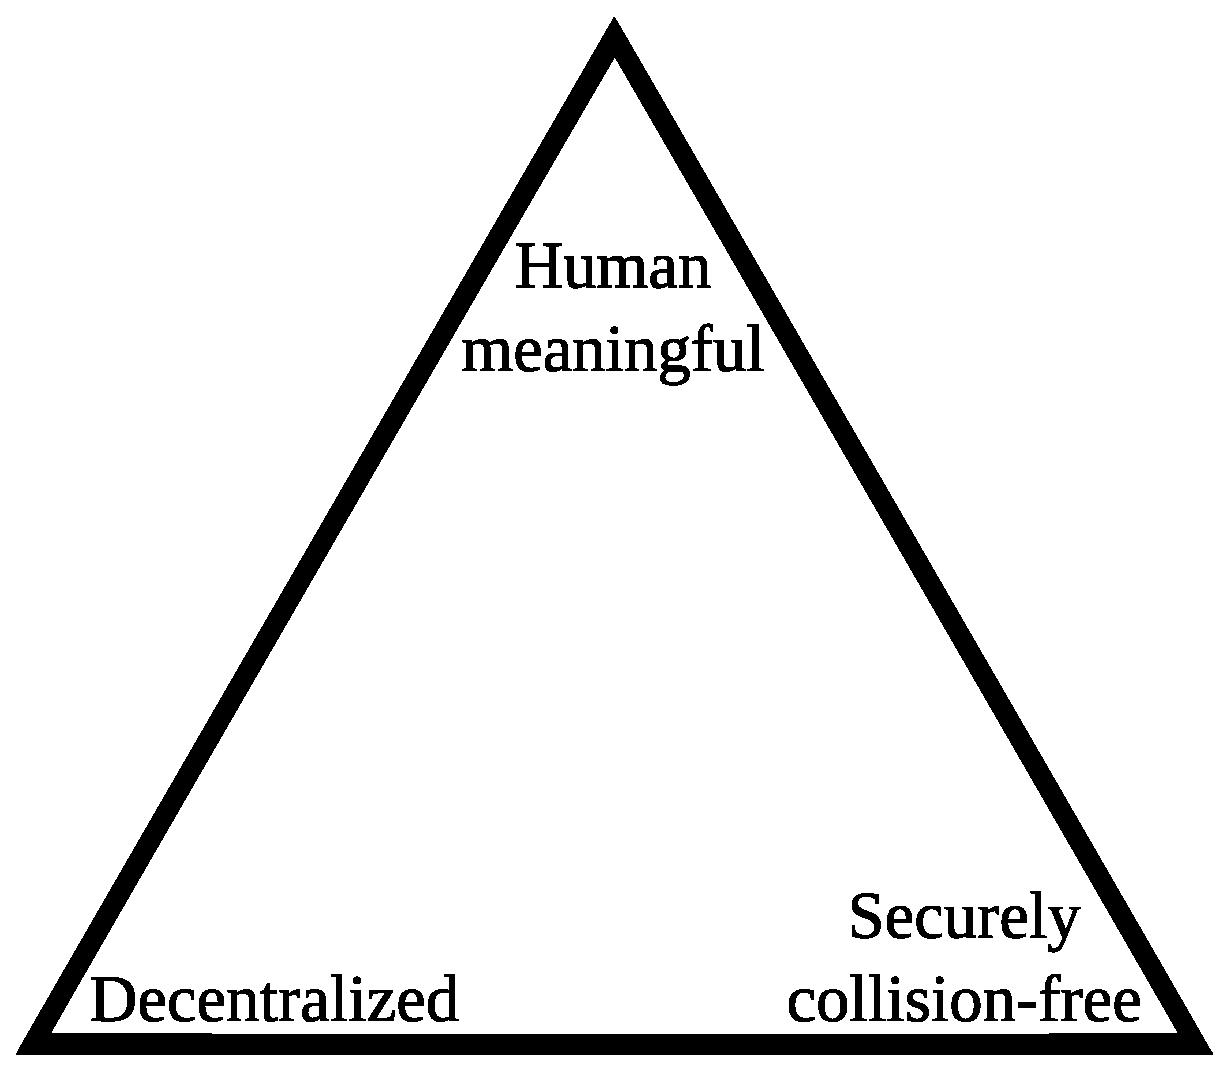
\includegraphics[width=0.3\textwidth]{../assets/images/Zooko.eps}
	\caption{Zooko's Triangle.}
	\label{fig:ZookosTriangle}
\end{figure}

\newpage

Some examples of naming systems that achieve only two of these properties include:

\begin{itemize}
	\item \textbf{Securely unique and human-meaningful} \\ --- Internet domain names and GNS.
	\item \textbf{Decentralized and human-meaningful} \\ --- Human names and nicknames.
	\item \textbf{Securely unique and decentralized} \\ --- Tor hidden service .onion addresses.
\end{itemize}

% Petnames, such as Namecoin and OnioNS, are systems that achieve all three properties of Zooko's Triangle.

\subsubsection{Authenticated Denial-of-Existence}
\label{sec:authDenialIntro}

If a naming system provides authentication, clients should be able to verify the authenticity of existing domain names and authenticate a denial-of-existence claim by their name server. On the Internet, the former is addressed by SSL certificates and a chain of trust to root Certificate Authorities, while the latter remains a possible attack vector. DNSSEC includes an extension for Hashed Authenticated Denial of Existence (NSEC3) which provides signed non-existence claims on a per-domain basis. However, DNSSEC has not seen widespread use, storing per-domain denial-of-existence records introduces significant storage requirements, and to our knowledge no alternative DNS provides mechanisms for authenticated denial-of-existence. Closing this attack vector is not easy; the na\"{i}ve solution of generating proof individually or en-masse for every non-existent domain is infeasible since the number of possible domain names is likely too large to practically enumerate.

\section{Related Works}
\label{sec:RelatedWorks}

Vanity key generators (e.g. Shallot\cite{KatmagicShallot}) attempt to find by brute-force an RSA key that generates a partially-desirable hash. Vanity key generators are commonly used by hidden service operators to improve the recognition of their hidden service, particularly for higher-profile services\cite{syversongenuine}. For example, a hidden service operator may wish to start his service's address with a meaningful noun so that others may more easily recognize it. However, these generators are only partially successful at enhancing readability because the size of the domain key-space is too large to be fully brute-forced in any reasonable length of time. If the address key-space was reduced to allow a full brute-force, the system would fail to be guaranteed collision-free. Nicolussi suggested changing the address encoding to a delimited series of words, using a dictionary known in advance by all parties\cite{nicolussi2011human}. Like vanity key generators, Nicolussi's encoding partially improves the recognition and readability of an address but does nothing to counter the large key-space nor alleviate the logistic problems of manually entering in the address into the Tor Browser. These attempts are purely cosmetic and do not qualify as a full solution.

The Internet DNS is another one candidate and is already well established as a fundamental abstraction layer for Internet routing. However, despite its widespread use and extreme popularity, the Internet DNS suffers from several significant shortcomings and fundamental security issues that make it inappropriate for use by Tor hidden services. Generally speaking, the Internet DNS by default does not use any cryptographic primitives. DNSSEC is primarily designed to prevent forgeries and DNS cache poisoning from intermediary name servers and it does not provide any degree of query privacy\cite{wachs2014censorship}. Additional extensions and protocols such as DNSCurve\cite{bernstein2009dnscurve} have been proposed, but DNSSEC and DNSCurve are optional and have not yet seen widespread full deployment across the Internet. The lack of default security in Internet DNS and the financial expenses involved with registering a new TLD casts significant doubt on the feasibility of using it for Tor hidden services. Cachin and Samar\cite{cachin2004secure} extended the Internet DNS and decreased the attack potential for authoritative name servers via threshold cryptography, but the lack of privacy in the Internet DNS and the logistical difficulty in globally implementing their work prevents us from using their system for hidden services.

The GNU Name System\cite{wachs2014censorship} (GNS) is another zone-based alternative DNS. GNS describes a hierarchical zones of names with each user managing their own zone and distributing zone access peer-to-peer within social circles. While GNS' design guarantees the uniqueness of names within each zone and users are capable of selecting meaningful nicknames for themselves, GNU does not guarantee that names are \emph{globally} unique. Furthermore, the selection of a trustworthy zone to use would be a significant challenge for using GNS for Tor hidden services and such a selection no longer makes the system distributed. Awerbuch and Scheideler,\cite{awerbuch2004group} constructed a distributed peer-to-peer naming system, but like GNS, made no guarantee that domain names would be globally unique.

% \cite{jacobs2014providing} was

Namecoin\cite{NamecoinHome} is an early fork of Bitcoin\cite{nakamoto2008bitcoin} and is noteworthy for achieving all three properties of Zooko's Triangle. Namecoin holds information transactions in a distributed ledger known as a blockchain. Storing textual information such as a domain registration consumes some Namecoins, a unit of currency. While Namecoin is often advertised as capable of assigning names to Tor hidden services, it has several practical issues that make it generally infeasible to be used for that purpose. First, to authenticate registrations, clients must be able to prove the relationship between a Namecoin owner's secp256k1 ECDSA key and the target hidden service's RSA key: constructing this relationship is non-trivial. Second, Namecoin generally requires users to pre-fetch the blockchain which introduces significant logistical issues due to high bandwidth, storage, and CPU load. Third, although Namecoin supports anonymous ownership of information, it is non-trivial to anonymously purchase Namecoins, thus preventing domain registration from being truly anonymous. These issues prevent Namecoin from being a practical alternative DNS for Tor hidden service. However, our work shares some design principles with Namecoin.

\section{Assumptions and Threat Model}
\label{sec:threatModel}

We assume that Tor provides privacy and anonymity; if Alice constructs a three-hop Tor circuit to Bob with modern Tor cryptographic protocols and sends a message $ m $ to Bob, we assume that Bob can learn no more about Alice than the contents of $ m $. This implies that if $ m $ does not contain identifiable information, Alice is anonymous from Bob's perspective, regardless of if $ m $ is exposed to an attacker, Eve. Identifiable information in $ m $ is outside of Tor's scope, but we do not introduce any protocols that cause this scenario. The security of Tor circuits is also dependent on the honesty of directory authorities: we also assume that more than fifty percent of Tor directory authorities are at least semi-honest; they may wiretap but are not capable of violating protocols. 

Let $ R $ be the set of Tor routers with the Fast, Stable, and Running flags and let $ Q $ be an $ M $-sized set randomly chosen from $ R $ with selection probability $ P (Q_{i}) = \frac{Q_{i}(w)}{\sum_{j=0}^{\concat R \concat} R_{j}(w)} $ where $ Q_{i}(w) $ is $ Q_{i} $'s consensus weight as determined by Tor directory authorities. We then assume that $ Q $ is under the influence of one or more adversaries and that largest subset of agreeing routers in $ Q $ are at least semi-honest.

%$ P (Q_{i}) = \frac{Q_{i}(w)}{\sum_{j=0}^{\concat R \concat} R_{j}(w)} $

We assume that Eve controls some percentage of dishonest colluding Tor routers as well as semi-honest routers, however this percentage is small enough to avoid violating our first assumption. We assume a fixed percentage of dishonest and semi-honest routers; namely that the percentage of routers under an Eve's control does not increase in response to the inclusion of OnionNS into Tor infrastructure. This assumption simplifies our threat model analysis but we consider it realistic because while Tor traffic is purposely secret as it travels through the network, we consider OnioNS information public so we don't consider the inclusion of OnioNS a motivating factor to Eve.

Finally, we assume secure cryptographic primitives; namely that Eve cannot break standard cryptographic primitives such as AES, SHA-2, RSA, Curve25519, Ed25519, and the scrypt key derivation function. We assume that Eve maintains no backdoors or knows secret software breaks in the Botan or the OpenSSL implementations of these primitives.

\section{Solution}
\label{sec:Solution}

\subsection{Overview}
\label{sec:SolutionOverview}

\begin{figure}[htbp]
	\centering
	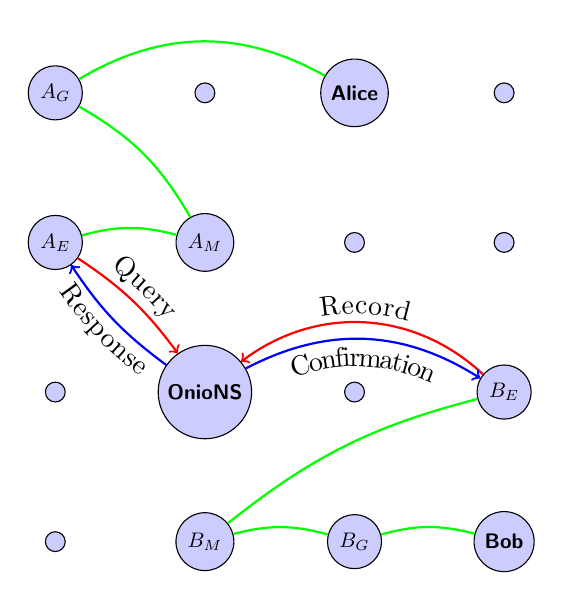
\begin{tikzpicture}[scale=0.76, ->, node distance=2.5cm, main node/.style={circle, fill=blue!20, draw, font=\sffamily\bfseries, transform shape}]

			\node[main node] (1) {$ A_{G} $};
			\node[main node] (2) [right of=1] {};
			\node[main node] (3) [right of=2] {Alice};
			\node[main node] (4) [right of=3] {};

			\node[main node] (5) [below of=1] {$ A_{E} $};
			\node[main node] (6) [right of=5] {$ A_{M} $};
			\node[main node] (7) [right of=6] {};
			\node[main node] (8) [right of=7] {};

			\node[main node] (9) [below of=5] {};
			\node[main node] (10) [right of=9] {OnioNS};
			\node[main node] (11) [right of=10] {};
			\node[main node] (12) [right of=11] {$ B_{E} $};

			\node[main node] (13) [below of=9] {};
			\node[main node] (14) [right of=13] {$ B_{M} $};
			\node[main node] (15) [right of=14] {$ B_{G} $};
			\node[main node] (16) [right of=15] {Bob};

			% Alice-OnioNS conversation
			\tikzstyle{EdgeStyle}=[bend right, -, green]
			\Edge[](3)(1)
			\tikzstyle{EdgeStyle}=[bend left=15, -, green]
			\Edge[](1)(6)
			\Edge[](5)(6)
			\draw[thick, ->, red, postaction={decorate, decoration={text along path, text align=center, text={Query}, raise=4pt}}] (5) to [bend left=10] (10){};
			\draw[thick, <-, blue, postaction={decorate, decoration={text along path, text align=center, text={Response}, raise=-9pt}}] (5) to [bend right=10] (10){};

			% Bob-OnioNS conversation
			\tikzstyle{EdgeStyle}=[bend right=15, -, green]
			\Edge[](16)(15)
			\Edge[](15)(14)
			\tikzstyle{EdgeStyle}=[bend left=12, -, green]
			\Edge[](14)(12)
			\draw[thick, red, <-, postaction={decorate, decoration={text along path, text align=center, text={Record}, raise=3pt}}] (10) to [bend left=40] (12){};
			\draw[thick, blue, ->, postaction={decorate, decoration={text along path, text align=center, text={Confirmation}, raise=-10pt}}] (10) to [bend left=30] (12){};

		\end{tikzpicture}
	\caption{Bob uses a Tor circuit ($ B_{G} $, $ B_{M} $, $ B_{E} $) to anonymously broadcast a record to OnioNS. Alice uses her own Tor circuit ($ A_{G} $, $ A_{M} $, $ A_{E} $) to query the system for a domain name, and she is given Bob's record in response. Then Alice connects to Bob by Tor's hidden service protocol.}
	\label{fig:basicDesign}
\end{figure}

We propose the Onion Name System (OnioNS) as an abstraction layer to hidden service addresses and introduce ``.tor'' as a new pseudo-TLD for this purpose. First, Bob generates and self-signs a \emph{Record}, containing a meaningful second-level domain name and his public key $ \mathcal{P}_{B} $. Without loss of generality, let this be ``example.tor $ \rightarrow $ onions55e7yam27n.onion''. We introduce a proof-of-work scheme that requires Bob to expend computational and memory resources to claim ``example.tor'', a more privacy-enhanced alternative to financial compensation to a central authority. Proof-of-work systems are noteworthy for their asymmetry: they require the issuer to spend effort to find an answer to a moderately hard computational problem, but once solved can be easily verified correct by any recipient. The requirement of proof-of-work fulfils three main purposes:

\begin{enumerate}
	\item Significantly reduces the threat of DoS flood attack.
	\item Introduces a barrier-of-entry that encourages the utilization of domain names and the availability of the underlying hidden services.
	\item Increases the difficulty of domain squatting.
\end{enumerate}

Second, Bob uses a Tor circuit to anonymously transmit his Record to an authoritative short-lived random subset of OnioNS servers, known as the Quorum, inside the Tor network. The Quorum archive Bob's Record in a sequential public ledger known as a Pagechain, of which each OnioNS node holds their own local copy. Bob's Record is received by all Quorum nodes and share signatures of their knowledge with each other, so they maintain a common database. Quorum nodes are not name servers, so let Charlie be a name server outside the Quorum and assume that Charlie stays synchronized with the Quorum.

Third, Alice, uses a Tor client to anonymously connect to Charlie, then asks Charlie for ``example.tor''. Alice receives Bob's Record, verifies its signature and proof-of-work, and uses $ \mathcal{P}_{B} $ to contact Bob via Tor's hidden service protocol. As Bob's Record is self-signed and contains $ \mathcal{P}_{B} $, Alice can verify the Record's authenticity relative to $ \mathcal{P}_{B} $. In this way, Alice does not have to resort to using ``onions55e7yam27n.onion'', rather that Bob can be successfully referenced by ``example.tor''. We illustrate the OnioNS overview in Figure \ref{fig:basicDesign}.

\subsection{Cryptographic Primitives}

OnioNS makes use of a number of cryptographic primitives, notably a proof-of-work algorithm and a global source of randomness. Additionally, we require that Tor routers generate an Ed25519\cite{bernstein2011high} keypair and distribute the public key via the consensus document. We note that because the Ed25519 elliptic curve is birationally equivalent to Curve25519\cite{bernstein2006curve25519} and because it is possible to convert Curve25519 to Ed25519 in constant time, we can theoretically use existing NTor\cite{goldberg2013anonymity} keys for digital signatures. However, we refrain from this because to our knowledge there is no formal analysis that demonstrates that this a cryptographically secure operation. Therefore we require Tor to introduce Ed25519 keys to all Tor routers. If this is infeasible, Ed25519 can be substituted with RSA in all instances.

\begin{itemize}
	\item Let $ \mathcal{H}(x) $ be a cryptographic hash function. In our reference implementation we define $ \mathcal{H}(x) $ as SHA-384.
	\item Let $ S_{\mathit{RSA}}(m, r) $ be a deterministic RSA digital signature function that accepts a message $ m $ and a private RSA key $ r $ and returns a digital signature. Let $ S_{\mathit{RSA}}(m, r) $ use $ \mathcal{H}(x) $ as a digest function on $ m $ in all use cases. In our reference implementation we define $ S_{\mathit{RSA}}(m, r) $ as EMSA PKCS1 v1.5. (EMSA3)
	\item Let $ V_{\mathit{RSA}}(m, R) $ validate an RSA digital signature by accepting a message $ m $ and a public key $ R $, and return true if and only if the signature is valid.
	\item Let $ S_{\mathit{ed}}(m, e) $ be an Ed25519 digital signature function that accepts a message $ m $ and a private key $ e $ and returns a 64-byte digital signature. Let $ S_{\mathit{ed}}(m, e) $ use $ \mathcal{H}(x) $ as a digest function on $ m $ in all use cases.
	\item Let $ V_{\mathit{ed}}(m, E) $ validate an Ed25519 digital signature by accepting a message $ m $ and a public key $ E $, and return true if and only if the signature is valid.
	\item Let $ \mathrm{PoW}(k) $ be a one-way function that accepts an input key $ k $ and returns a deterministic output. Our reference implementation uses the scrypt\cite{percival2012scrypt} key derivation function with a fixed salt.
	\item Let $ \mathcal{G}(t) $ be a cryptographically-secure generator of random or pseudorandom timestapped numbers. $ \mathcal{G}(t) $ deterministically returns a value for time $ t $ in the present or past.
	\item Let $ \mathcal{R}(s) $ be a pseudorandom number generator that accepts an initial seed $ s $ and returns a list of pseudorandom numbers. In our design, $ \mathcal{R}(s) $ uses $ \mathcal{G}(t) $, so $ \mathcal{R}(s) $ does not need to be cryptographically secure. We suggest MT19937, commonly known as the Mersenne Twister. This generator is widely used throughout most programming languages and is well known for its speed, long period, and the high quality of its pseudorandom output\cite{matsumoto1998mersenne}.
\end{itemize}

\subsection{Definitions}

\textbf{domain name} The syntax of OnioNS domain names mirrors the Internet DNS; we use a sequence of name-delimiter pairs with a .tor pseudo-TLD. The Internet DNS defines a hierarchy of administrative realms that are closely tied to the depth of each name. By contrast, OnioNS makes no such distinction; we let hidden service operators claim second-level names and then control all names of greater depth under that second-level name.

A \textbf{Record} contains $ \mathit{type} $, the purpose of this Record; $ \mathit{name} $, a meaningful second-level domain name with the .tor pseudo-TLD; $ \mathit{subdomains} $, a one-to-one map of .tor domains of level three or higher and .tor or .onion destinations; $ \mathit{contact} $, Bob's PGP key fingerprint if he chooses to disclose it; $ \mathit{rand} $, the output of $ \mathcal{G}(t) $ at the current time; $ \mathit{nonce} $, bytes used as a source of randomness for the proof-of-work; $ \mathit{pow} $, the output of $ \mathrm{PoW}(i) $;  $ \mathit{signature} $, the output of $ S_{\mathit{RSA}}(m, r) $; and $ \mathit{pubHSKey} $, Bob's public RSA key.

A \textbf{Page} contains $ \mathit{prevHash} $, set to $ \mathcal{H}(\mathit{prevHash} \concat \mathit{recordList} \concat \mathit{rand}) $ of some previous Page; $ \mathit{recordList} $, a \\ deterministically-sorted array list of Records; $ \mathit{rand} $, the output of $ \mathcal{G}(t) $ at the current time; $ \mathit{fingerprint} $, the Tor fingerprint of the router maintaining this Page; and $ \mathit{pageSig} $, the output of  $ S_{\mathit{ed}}(\mathcal{H}(\mathit{prevHash} \concat \mathit{recordList} \concat \mathit{rand}), e) $ where $ e $ is the router's private Ed25519 key.

$ \mathit{prevHash} $ links Pages over time, forming an append-only public ledger known as a Pagechain. In contrast to existing cryptocurrencies such as Namecoin, we bound the Pagechain to a finite length, forcing hidden service operators to renew their domain periodically to avoid it being dropped from the network. In correspondence with our security assumptions, $ \mathit{prevHash} $ must reference a Page that is both valid and maintained by the largest number of Quorum members whom we assume are at least semi-honest, as illustrated in Figure \ref{fig:sideChains}. As $ \mathit{prevHash} $ does not include the router-specific $ \mathit{fingerprint} $ and $ \mathit{pageSig} $ fields, $ \mathit{prevHash} $ is equal across all Quorum members maintaining that Page.

A \textbf{Mirror} is any name server that holds a complete copy of the Pagechain and maintains synchronization against the Quorum. Mirrors respond to queries but must provide signatures from Quorum nodes to prevent Mirrors from falsifying responses. We note that Mirrors may be outside the Tor network, but in this work we do not specify any protocols for this scenario.

\textbf{Quorum Candidate} are \emph{Mirrors} that provide proof in the network status consensus that they are an up-to-date Mirror in the Tor network and that they have sufficient CPU and bandwidth capabilities to handle OnioNS communication in addition to their Tor duties.

A \textbf{Quorum} is a subset of Quorum Candidates who have active responsibility over maintaining the master Pagechain. Each Quorum node actively maintains its own Page, which has a lifetime of that Quorum. The Quorum is randomly chosen from Quorum Candidates as described in section \ref{sec:qFormation}.

\begin{figure}[h]
	\centering
	\includegraphics[width=0.7\linewidth]{../assets/images/LucidCharts/Page-chain2.pdf}
	\caption{An example Pagechain across four Quorums with three side-chains. The valid master Pagechain from honest/semi-honest Quorum nodes (green) resists corruption from dishonest and colluding nodes (red) and malfunctioning nodes (orange).}
	\label{fig:sideChains}
\end{figure}

%\setlength{\belowcaptionskip}{-10pt}
\begin{figure}[h!]
	\centering
	\includegraphics[width=0.9\linewidth]{../assets/images/LucidCharts/Data-Structure-Overview.pdf}
	\caption{The master Pagechain is one-dimensional but spans across the network as each Mirror holds a copy. Each Page is maintained by a respective Quorum.}
\end{figure}

\renewcommand{\arraystretch}{1.2}
\begin{table}[h]
	\small
	\begin{tabularx}{\linewidth}{ | l | X | }
		\hline
    	$ L_{Q} $ & the size of the Quorum \\ \hline
    	$ L_{T} $ & the number of routers in the Tor network \\ \hline
    	$ L_{P} $ & the maximum number of Pages in the Pagechain \\ \hline
    	$ q $ & the Quorum iteration counter \\ \hline
    	$ \Delta q $ & the lifetime of a Quorum in days \\ \hline
  	\end{tabularx}
  	\vspace{6pt}
  	\caption{Frequently used notations}
\end{table}

\subsection{Protocols}

We now describe the protocols fundamental to OnioNS functionality.

\subsubsection{Random Number Generation}

We use $ \mathcal{G}(t) $ as a basis for Quorum selection, although we note that $ \mathcal{G}(t) $ has applications in Tor beyond OnioNS. One straightforward definition of $ \mathcal{G}(t) $ is the SHA-384 hash of Tor's consensus documents. If the Tor network is dynamic enough to provide significant amounts of entropy into the consensus documents, then $ \mathcal{G}(t) $ may be considered cryptographically secure. However, this assumption does not hold because current router descriptors are publicly available before the consensus documents are published, allowing $ \mathcal{G}(t) $ under this approach to be easily manipulated by a few malicious Tor routers. The attack becomes significantly easier in the final moments before the directory authorities publish the consensus.

Instead, we suggest implementing $ \mathcal{G}(t) $ as the commitment scheme proposed by Goulet and Kadianakis\cite{GouletCommitReveal}. Their algorithm modifies the consensus voting protocol that is run once an hour by Tor directory authorities. In their scheme, each authority commits a SHA-256 hash of a secret key $ x $ into each consensus vote across a 12 hour period. Then each directory authority reveals $ x $ across the next set of 12 consensuses. Finally, the revealed values are hashed together to create a single random number, which is then embedded in the consensus documents so that it is efficiently distributed to both Tor router and end users. A different random number thus appears in the consensus every 24 hours. We reiterate their security analysis in section \ref{sec:RandGeneration}.

\subsubsection{Quorum Qualification}

Quorum Candidates must prove that they are both up-to-date Mirrors and that they sufficient capabilities to handle the increase in communication and processing from OnioNS protocols.

The na\"{i}ve solution to demonstrating the first requirement is to simply ask Mirrors for their Page, and then compare the recency of its latest Page against the Pages from the other Mirrors. However, this solution does not scale well; Tor has $ \approx $ 2.1 million daily users\cite{TorMetrics}: it is infeasible for any single node to handle queries from all of them. Instead, let each Mirror first calculate $ t = \mathcal{H}(\mathit{pc} \concat \floor[\big]{\frac{m - 15}{30}}) $ where \emph{pc} is the Mirror's Pagechain and $ m $ is the number of minutes elapsed in that day, then include $ t $ in the Operator Contact field in his relay descriptor. Tor's consensus documents are published at the top of each hour; we manipulate $ m $ such that $ t $ is consistent at the top of each hour even with at most a 15-minute clock-skew. We suggest placing $ t $ inside a new field within the router descriptor in future work, but our use of the Contact field eases integration with existing Tor infrastructure. OnionNS would not be the first system to embed special information in the Operator Contact field: PGP keys and BTC addresses commonly appear in the field, especially for high-performance routers.

Tor's infrastructure already provides a mechanism for demonstrating the latter requirement; Quorum Candidates must also have the Fast, Stable, and Running flags. Tor routers with higher CPU or bandwidth capabilities relative to their peers also receive a proportionally larger consensus weight from the directory authorities. This consensus weight in turn strongly influences router selection during circuit construction: routers with higher weights are more likely to be chosen in a circuit. Thus, we can benefit from this infrastructure by selecting the Quorum from the pool of Quorum Candidates by a similar mechanism.

%mention that consensus weight is tied to path selection

\subsubsection{Quorum Formation}
\label{sec:qFormation}

Quorum Candidates and Tor clients can derive a Quorum in $ \mathcal{O}(L_{T}) $ time. Without loss of generality, let Alice run this algorithm.

\begin{enumerate}
	\item Alice obtains the consensus documents, $ \mathit{cd} $, published on day $ \floor[\big]{\frac{q}{\Delta q}} $ at 00:00 UTC.
	\item Alice extracts $ g = \mathcal{G}(t) $ from $ cd $.
	\item Alice scans $ \mathit{cd} $ and constructs a list $ l $ of Quorum Candidates that have the Fast, Stable, and Running flags and that are in the largest set of Tor routers that publish an identical time-based hash.
	\item Alice computes $ s = \sum_{j=0}^{\concat l \concat} l_{j}(w) $ where $ l_{j}(w) $ is $ l_{j} $'s consensus weight as determined by Tor directory authorities.
	\item Alice uses $ \mathcal{R}(g) $ to select $ \mathrm{min}(\mathrm{size}(l), L_{Q}) $ Quorum nodes from $ l $ with selection probability \\ $ P (Q_{i}) = \frac{Q_{j}(w)}{s} $.
\end{enumerate}

This procedure may be performed on any $ \mathit{cd} $ in the past because Tor consensus documents contain timestamps and digital signatures from Tor directory authorities and thus may be retroactively verified regardless of where they are archived.

\subsubsection{Record Generation}
\label{sec:RecordGeneration}

Bob must first generate a valid Record to claim a second-level domain name for his hidden service. The validity of his Record is checked by Mirrors and clients, so Bob must follow this protocol to ensure that his Record is accepted.

\begin{enumerate}
	\item Bob sets \emph{type} to ``Create''.
	\item Bob provides the \emph{name} and \emph{subdomains} fields by specifying a second-level domain name and subdomain-destination pairs for his hidden service, respectively.
	\item Bob optionally sets \emph{contact} to his PGP key fingerprint.
	\item Bob sets \emph{rand} to the value from $ \mathcal{G}(t) $ as published in the consensus documents on day $ \floor[\big]{\frac{q}{\Delta q}} $ at 00:00 UTC.
	\item Bob fills \emph{nonce} with zeros.
	\item Let $ \mathit{c} $ be $\mathit{type} \concat \mathit{name} \concat \mathit{subdomains} \concat \mathit{contact} \concat \mathit{rand} \concat \mathit{nonce} $.
	\item Bob sets \emph{pow} as $ \mathrm{PoW}(\mathit{c}) $.
	\item Bob sets \emph{signature} as the output of $ S_{\mathit{RSA}}(m, r) $ where $ m = \mathit{c} \concat \mathit{pow} $ and $ r $ is Bob's private RSA key.
	\item Bob saves the PKCS.1 DER encoding of his RSA public key in \emph{pubHSKey}.
\end{enumerate}

The Record is valid when $ \mathcal{H}(\mathit{c} \concat \mathit{pow} \concat \mathit{signature}) \leq d $ where \emph{d} is a fixed constant that specifies the work difficulty. This also requires Bob to increment \emph{nonce} and resign his Record at every iteration of $ \mathrm{PoW}(\mathit{c}) $. Once it is valid, Bob can send his Record to all Quorum nodes.

\subsubsection{Record Operations}

The Onion Name System also supports common operations on Records in a manner similar to Namecoin. So long as Bob retains exclusive knowledge of his private key, he may manipulate his own Records at any later date.

\textbf{Modification} Although Bob cannot change the Record's \emph{name} field, he can change the \emph{subdomains} or \emph{contact} fields by reissuing another Record with these manipulations in place. This modification requires a difficulty of $ \frac{d}{4} $.

\textbf{Deletion} To relinquish his claim, he may issue a deletion record, releasing his domain and allowing it to be claimed by another. There is no difficulty in doing this, so his request can be issued immediately, which may be beneficial in some cases.

\textbf{Renew} Bob must also periodically renew his claim by reissuing his Record every $ L_{P} * \Delta q $ days to ensure that the Page containing it does not drop off the Pagechain. This requires the same difficulty as generating a new Record.

\textbf{Transfer} Bob may also choose to change the ownership of his Record. He can do this by issuing a transfer Record, which includes a new field, \emph{recipientKey}, the public RSA key of the recipient. However, unlike Namecoin, here Bob also retains the ability to issue a deletion Record. This property not only discourages the economic benefits of domain squatting, but also helps provides a defence against phishing attacks. If Eve gains access to Bob's private key and issues a transfer Record to her key before Bob notices the breach, Bob can still release the domain to minimize the impact.

\subsubsection{Record Processing}

A Quorum node $ Q_{j} $ listens for new Records from hidden service operators. Mirrors subscribe to Quorum nodes by maintaining a network session with them and sending a subscription request. This allows Records to traverse the network quickly in a peer-to-peer fashion. When a Record $ r $ is received, $ Q_{j} $

\begin{enumerate}
	\item $ Q_{j} $ rejects $ r $'s \emph{name} already exists in $ Q_{j} $'s Pagechain.
	\item $ Q_{j} $ rejects $ r $ if the Record is not valid according to the above protocol.
	\item $ Q_{j} $ rejects $ r $ if Bob's hidden service or any destination in \emph{subdomains} does not exist.
	\item $ Q_{j} $ informs Bob that $ r $ has been accepted.
	\item $ Q_{j} $ sends $ r $ to all of its subscribers.
\end{enumerate}

Quorum nodes must also periodically regenerate and resign the Merkle tree described in \ref{sec:authDenial} and send the signature to all Quorum nodes and to all subscribers.

\subsubsection{Page Selection}

New Quorum nodes must select a Page from the previous Quorum to reference when generating a fresh Page. To reduce the chances of compromise, we select Pages according to our security assumptions. Let Charlie be a Mirror.

\begin{enumerate}
	\item Charlie obtains and authenticates the consensus \emph{cd} issued on day $ \floor[\big]{\frac{q}{\Delta q}} $ at 00:00 UTC and authenticates it.
	\item Charlie derives the Quorum via the procedure described in section \ref{sec:qFormation}.
	\item Charlie obtains the set of Pages maintained by $ \mathit{Quorum}_{q} $.
	\item For each Page,
		\begin{enumerate}
			\item Charlie asserts that $ \mathit{fingerprint} \in \mathit{Quorum}_{q} $.
			\item Charlie asserts that \emph{prevHash} references $ \mathrm{Page}_{q-1} $ found by this protocol.
			\item Charlie calculates $ h = \mathcal{H}(\mathit{prevHash} \concat \mathit{recordList} \concat \mathit{rand}) $.
			\item Charlie asserts that $ V_{\mathit{ed}}(h, E) $ returns true.
		\end{enumerate}
	\item Charlie sorts the set of Pages by the number of routers that have signed $ h $.
	\item For each Page in each $ h $,
		\begin{enumerate}
			\item Charlie checks that \emph{rand} is contained in \emph{cd}.
			\item Charlie checks the validity of each Record in \emph{recordList}.
		\end{enumerate}
	\item If the validation of a Page fails, Charlie continues to the next $ h $.
	\item If the Page is valid, Charlie selects this page and aborts the procedure.
\end{enumerate}

\subsubsection{Domain Query}

Alice needs only Bob's Record to contact Bob by his meaningful domain name. Let Alice type a domain $ d $ into the Tor Browser.

\begin{enumerate}
	\item Alice constructs a Tor circuit to Charlie.
	\item \label{step:ask} Alice asks Charlie for the most recent Record $ r $ containing $ d $.
	\item Charlie finds and returns $ r $ to Alice and the components of the Merkle tree $ T $ described in section \ref{sec:authDenial}.
	\item If $ r $ is not found, Alice asserts that the second-level name of $ d $ is not found in $ T $, as otherwise Charlie is dishonest.
	\item If $ r $ is found, Alice asserts that $ r $ is valid and contained in $ T $, as otherwise Charlie is dishonest.
	\item If $ d $ in $ r $ points to a domain with a .tor pseudo-TLD, $ d $ becomes that destination and Alice jumps to step \ref{step:ask}.
	\item Alice asserts that the destination uses a .onion pseudo-TLD and contacts Bob by the traditional hidden service protocol.
	\item Alice extracts Bob's key from his hidden service descriptor and asserts that it matches $ r $'s \emph{pubHSKey}.
	\item Alice sends the original $ d $ to the hidden service.
\end{enumerate}

The Merkle tree also prevents phishing attacks from Charlie. While the Quorum provides the verification that $ r $ is authentic and that $ d $ is unique, Alice may become certain by performing a synchronization against the OnioNS network and checking the Pagechain herself, but this is impractical in most environments. Tor's median circuit speed is often less than 4 Mbit/s,\cite{TorMetrics} so for the sake of convenience data transfer must be minimized. Therefore Alice can simply fetch minimal information and rely on her existing trust of members of the Tor network.

\subsubsection{Onion Query}

OnioNS also supports reverse-hostname lookups. In an Onion Query, Alice issues a hidden service address \emph{addr} to Charlie and receives back all Records that have \emph{addr} as either the owner or as a destination in their \emph{subdomain}. Alice may obtain additional verification on the results by issuing Domain Queries on the source .tor domains. We do not anticipate Onion Queries to have significant practical value, but they complete the symmetry of lookups and allow OnioNS domain names to have Forward-Confirmed Reverse DNS matches. We suggest caching destination hidden service addresses in a digital tree (trie) to accelerate this lookup; a trie turns the lookup from $ \mathcal{O}(n) $ to $ \mathcal{O}(1) $, while requiring $ \mathcal{O}(n) $ time and $ \mathcal{O}(n) $ space to pre-compute the cache.

\subsection{Authenticated Denial-of-Existence}
\label{sec:authDenial}

In any system that serves authenticable names, a name server can prove a claim on the existence of a name by simply returning it. An often overlooked problem is ensuring that name servers cannot claim false negatives on resolutions; clients must be able to authenticate a denial-of-existence claim. Extensions to DNSSEC attempt to close this attack vector, but DNSSEC is not widely deployed, and we are not aware of any alternative DNS that addresses this. Although Alice may download the entire Pagechain and prove non-existence herself, we do not consider this approach practical in most realistic environments. Instead, we introduce a mechanism for authenticating denial-of-existence with minimal networking costs. To our knowledge this represents the first alternative DNS to authenticate denial-of-existence claims on domains en-masse.

We suggest reducing the networking costs with a Merkle tree\cite{merkle1988digital} $ T $. Let each Quorum node

\begin{enumerate}
	\item Construct an array list \emph{arr}.
	\item For each second-level domain $ c $ in each Record $ r $ in the Pagechain, add $ c \concat \mathcal{H}(r) $ to \emph{arr}.
	\item Sort \emph{arr}.
	\item Construct a Merkle tree $ T $ from \emph{arr}.
	\item Generate $ \mathit{sig}_{T} = S_{\mathit{ed}}(t \concat r, e) $ where $ t $ is a timestamp and $ r $ is the root hash of $ T $.
\end{enumerate}

As Records contain both second-level domains and their subdomains, $ T $ needs only contain $ c $ to reference all domains in $ r $, which further saves space. Then during a Domain Query Alice may use $ T $ to authenticate a domain $ d $ and verify non-existence for a Record $ r $.

\begin{enumerate}
	\item Alice extracts the second-level name $ c $ from $ d $.
	\item If $ r $ exists, Charlie returns the leaf node containing $ r $ and all the tree nodes from leaf $ r $ to the root and their sibling nodes, so that Alice can verify authenticity of $ r $ by recomputing the root hash and verify that the largest subset of Quorum nodes signed the same root hash.
	\item If Charlie claims non-existence of $ c $, he returns two adjacent leaves $ a $ and $ b $ (and the nodes on their paths and siblings) such that $ a < c < b $, or in the boundary cases that $ a $ is undefined and $ b $ is the left-most leaf or $ b $ is undefined and $ a $ is the right-most leaf.
	\item If either assertion fails, Charlie is dishonest.
\end{enumerate}

The Quorum must regenerate $ T $ every $ \Delta T $ hours to include new Records. Then Alice needs only fetch the signatures on $ T $ at least every $ \Delta T $ hours to ensure that she can authenticate new Records during the Domain Query. Thus $ \Delta T $ is the primary factor in the speed of Record propagation: Alice cannot authenticate or verify denial-of-existence claims on Records newer than $ \Delta T $. Alice must also fetch the $ L_{Q} $ signature from all Quorum nodes and assert that $ T $ is signed by the largest set of nodes maintaining the same Page, in correspondence with our security assumptions.

We note that a sorted Merkle tree does not support efficient dynamic record updates. The tree needs to be rebuilt to handle updates. To support efficient record update in $ \mathcal{O}(\mathrm{log}(n)) $ time, we can adopt the skip list data structure proposed in \cite{goodrich2001implementation}. Proof of existence and non-existence still works in a similar way.

\section{Security Analysis}
\label{sec:Analysis}

In this section, we analyse the security of the OnioNS system with regard to our security goals. First, the registrations and client queries are anonymous because they occur over a Tor circuit, which we assume provides privacy and anonymity. No identifiable information is leaked from the data contents as well. Second, registrations are authenticable, which can be reduced to the security of the Merkle hash tree and to the assumption that the largest subset of Quorum nodes are honest. We verify this assumption in section \ref{sec:QSelection} and \ref{sec:qSize}. Domain uniqueness also stems from the above assumption, relying on honesty of Quorum nodes to avoid collisions. Quorum selection is a random process assuming security of the commitment algorithm run by the directory authorities, which we analyse in section \ref{sec:RandGeneration}. We also highlight the potential for the leakage of the .tor pseudo-TLD on the Internet DNS.

\subsection{Quorum Selection}
\label{sec:QSelection}

In section \ref{sec:threatModel}, we assume that an attacker, Eve, controls some fixed $ f_{E} $ fraction of routers on the Tor network. Quorum selection may be considered as an $ L_{Q} $-sized random sample taken from an $ L_{T} $-sized population without replacement, where the population contains $ L_{T} * f_{E} $ entities that we assume are compromised and colluding. If our selection includes $ L_{E} $ Eve-controlled routers, then Eve controls the Quorum if either $ > \frac{L_{Q} - L_{E}}{2} $ honest Quorum nodes disagree or if $ L_{E} > \frac{L_{Q}}{2} $. The former scenario is hard to model theoretically or in simulation, but the probability of the latter can be statistically calculated. The Quorum is rotated every $ \Delta q $ days, so we must consider the implications of selections for both $ L_{Q} $ and $ \Delta q $.

\subsubsection{Quorum Size}
\label{sec:qSize}

The probability that Eve controls $ L_{E} $ Quorum nodes is given by the hypergeometric distribution, whose probability mass function (PMF) is shown in Equation \ref{eq:hypergeoPMF}.

\begin{align}
	\mathrm{Pr}(L_{E}) &= \frac{\binom{L_{T} * f_{E}}{L_{E}}\binom{L_{T} - L_{T} * f_{E}}{L_{Q} - L_{E}}}{\binom{L_{T}}{L_{Q}}}
	\label{eq:hypergeoPMF}
	\\
	\mathrm{Pr}(L_{E} > \frac{L_{Q}}{2}) &= \displaystyle\sum_{x=\ceil{\frac{L_{Q}}{2}}}^{L_{Q}} \frac{\binom{L_{T} * f_{E}}{x}\binom{L_{T} - L_{T} * f_{E}}{L_{Q} - x}}{\binom{L_{T}}{L_{Q}}}
	\label{eq:compromiseProb}
\end{align}

If all Quorum Candidates have an equal probability of selection, then the probability that $ L_{E} > \frac{L_{Q}}{2} $ is given by the $p$-value of the hypergeometric test for over-representation, expressed in Equation \ref{eq:compromiseProb}. Odd choices for $ L_{Q} $ prevents the network from splintering in the event that the Quorum is evenly split across two Pages. We provide the statistical calculations of Equation \ref{eq:compromiseProb} for various Quorum sizes in Figure \ref{fig:quorumUnweightedMajority}.

\begin{figure}[htbp]
	\centering
	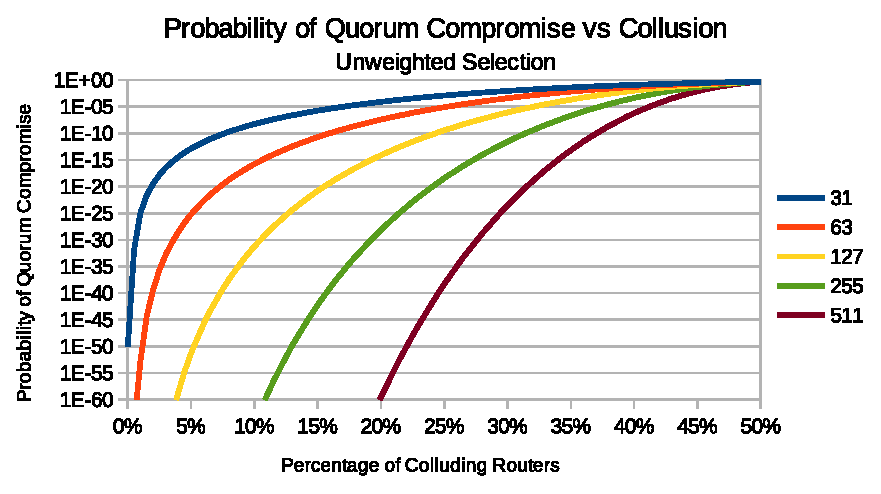
\includegraphics[width=\linewidth]{../assets/analysis/QuorumSelectionUnweighted.eps}
	\caption{The values for $ \mathrm{Pr}(L_{E} > \frac{L_{Q}}{2}) $ for Quorum sizes of 31, 63, 127, 255, and 511. All probabilities exceed 0.5 when more than 50 percent of the Tor network is under Eve's control. We set our population to 4540 routers; the average number of routers with the Fast, Stable, and Running flags across all consensuses in July 2015\cite{TorMetrics}.}
	\label{fig:quorumUnweightedMajority}
\end{figure}

In practice Tor routers do not have equal consensus weight, thus Quorum selection from the pool of Quorum Candidates is heavily skewed by the distribution of consensus weight. The selection probabilities of routers with the Fast, Stable, and Running flags closely follows an exponentially-decreasing distribution, as shown in Figure \ref{fig:weightDist}. The figure suggests that the Tor network contains a low number of high-end routers and a large number of low-end routers.

\begin{figure}[htbp]
	\centering
	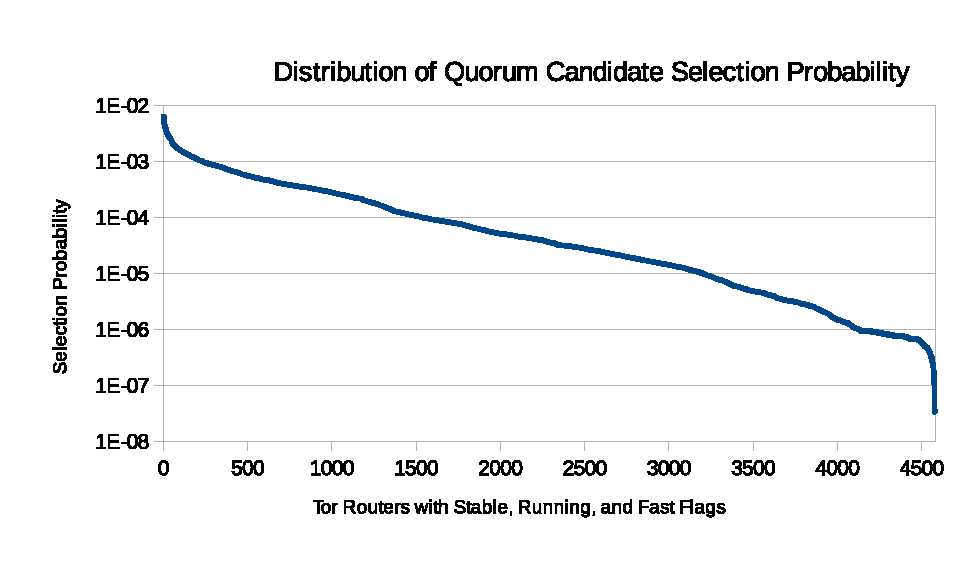
\includegraphics[width=\linewidth]{../assets/analysis/QuorumCandidateWeights.eps}
	\caption{The selection probabilities of Quorum Candidates averaged across all consensuses in July 2015. The probability of selecting each router is its consensus weight divided by the weights of all other Quorum Candidates. These probabilities closely follow an exponential distribution; a exponential trendline models it with $ R^{2} = 0.9884 $.}
	\label{fig:weightDist}
\end{figure}

We re-examine Equation \ref{eq:compromiseProb} with regard to this distribution of consensus weight in Figure \ref{fig:quorumWeightedMajority}. In contrast to Figure \ref{fig:quorumUnweightedMajority} which demonstrates that an unweighted selection leads to a high probability of compromise with small levels of collusion, Figure \ref{fig:quorumWeightedMajority} suggests that biasing Quorum selection by consensus weight provides a strong defence against large-scale Sybil attacks. Indeed, even when 60 percent of the low-end Quorum Candidates are malicious, most Quorum sizes produce negligible probabilities of compromise. We consider it reasonable to assume that low-end routers are under Eve's control; these routers are the cheapest and logistically easiest to operate. Our approach remains resistant to this attack: these routers will be included in the Quorum very infrequently because of their low consensus weight.

\begin{figure}[htbp]
	\centering
	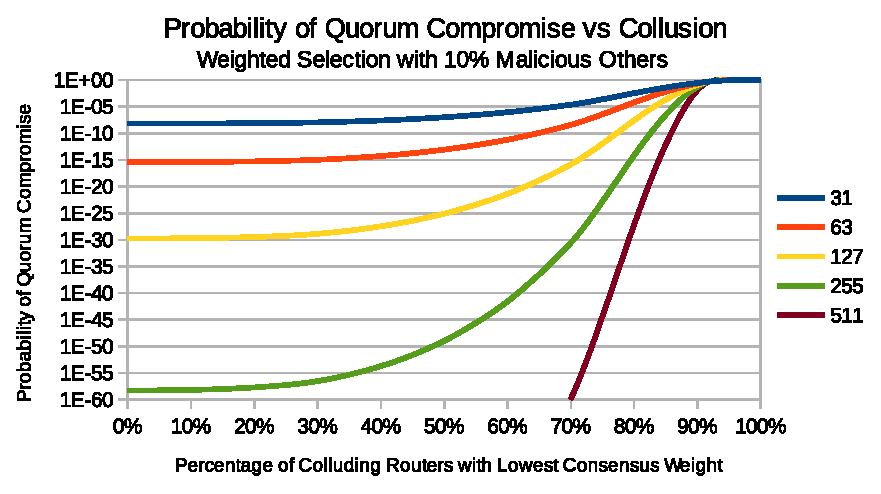
\includegraphics[width=\linewidth]{../assets/analysis/QuorumSelectionWeighted10.eps}
	\caption{The values for $ \mathrm{Pr}(L_{E} > \frac{L_{Q}}{2}) $ for various Quorum sizes. We assume that all routers with weights in the lowest X percentile are under Eve's control, while all other routers have a 10 percent chance of being under Eve's influence.}
	\label{fig:quorumWeightedMajority}
\end{figure}

Small Quorums are also more susceptible to node downtime or distributed denial-of-service (DDoS) attacks. Figure \ref{fig:quorumWeightedMajority} shows that the choices of $ L_{Q} = 31 $ is suboptimal; it is more easily compromised even with low levels of collusion. $ L_{Q} = 63 $ is more resistant, but not significantly more so. We therefore recommend $ L_{Q} \geq 127 $.

\subsubsection{Quorum Rotation}

In section \ref{sec:threatModel}, we assume that $ f_{E} $ is fixed and does not increase in response to the inclusion of OnioNS on the Tor network. If we also assume that $ L_{T} $ is fixed, then we can examine the impact of choices for $ \Delta q $ and calculate the probability of Eve compromising \emph{any} Quorum over a long period of time $ t $. Smaller values for $ \Delta q $ implies that we select more Quorums over that time period and thus increase our cumulative chances of compromise, but it also reduces the disruption timeline for a malicious Quorum. Eve's cumulative chances of compromising any Quorum is given by $ 1 - (1 - f_{c})^{\frac{t}{\Delta q}} $ where $ f_{c} $ is Eve's chances of compromising a single Quorum. We estimate this over 10 years in Figure \ref{fig:cumulativeProbability}.

\begin{figure}[h]
	\centering
	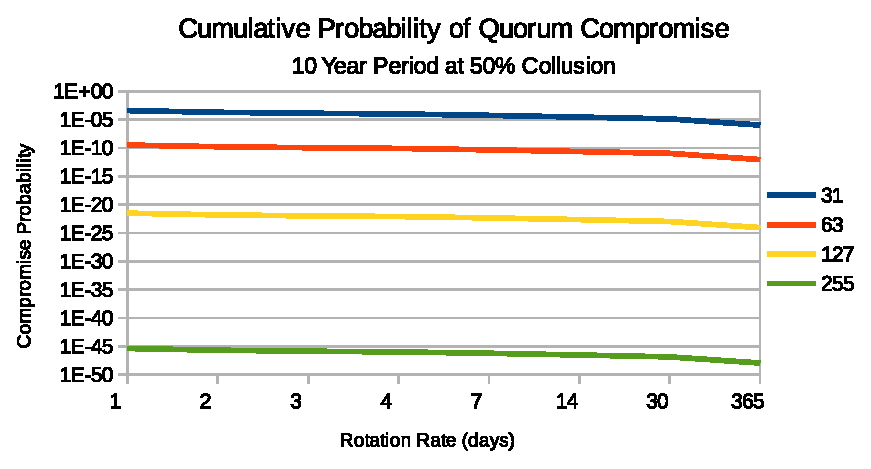
\includegraphics[width=\linewidth]{../assets/analysis/CumulativeMaliciousQuorumNew.eps}
	\caption{The cumulative probability that Eve controls any Quorum at different rotation rates over 10 years at $ f_{E} = 50 $ for Quorum sizes 31, 63, 127, and 255. We base these statistics on the probabilities from Figure \ref{fig:quorumWeightedMajority} at 50 percent collusion.}
	\label{fig:cumulativeProbability}
\end{figure}

%It also supports our earlier conclusion that the choices of $ L_{Q} = 31 $ and $ L_{Q} = 63 $ are suboptimal.
Figure \ref{fig:cumulativeProbability} suggests that although lower values of $ \Delta q $ negatively impact security, the choice of $ L_{Q} $ is more significant. Based on Figure \ref{fig:cumulativeProbability} we further reiterate our recommendation of $ L_{Q} \geq 127 $ and suggest $ \Delta q = 7 $. Although a malicious Quorum would have the capabilities to deploy a variety of attacks on the network, the proper selections of $ L_{Q} $ and $ \Delta q $ reduces the likelihood of this occurring to near-zero probabilities. We consider this a stronger solution than introducing countermeasures to specific Quorum-level attacks.

\subsubsection{Global Randomness}
\label{sec:RandGeneration}

We implement $ \mathcal{G}(t) $ using a commitment scheme run by Tor directory authorities\cite{GouletCommitReveal}. Commitment protocols have been studied in other works\cite{rivest1999unconditionally}\cite{naor1990bit}, have many interesting applications, and are well understood. If all parties are at least semi-honest then the commitment protocols generally display correctness, privacy, and binding. 

However, if some participants are malicious, they demonstrate known weaknesses. Namely, while reveals must demonstrably match commits, each participant may choose to reveal or not. If they do not reveal, their value is lost and the protocol produces a different output. If Eve controls $ b $ participants, she can make this choice with each participant in turn, allowing $ 2^{b} $ different outcomes. Goulet and Kadianakis' directory authority commitment scheme is particularly vulnerable to this attack because the reveals are public for approximately 12 hours before the final random value is published. However, as there are currently only nine directory authorities and the security of the Tor network rests on the assumption that five or more of them are at least semi-honest, the commitment scheme has at most $ 2^{4} = 16 $ different outcomes in the worst case without violation of our assumptions. 

Given the statistical calculations and the safety margin introduced by the recommendations in section \ref{sec:qSize}, we do not consider this a significant threat to our system and conclude that the Quorum Formation protocol is secure under our design assumptions. The unpredictability of the reveals and the low probability of compromise shown in Figures \ref{fig:quorumWeightedMajority} and \ref{fig:cumulativeProbability} provides the strongest defence against Quorum-level attacks.

\subsection{Outsourcing Record Generation}

In the Record Generation protocol, we intentionally included the scrypt calculation inside the signing step in order to require Bob to run scrypt himself. However, our protocol does not entirely prevent Bob from outsourcing this expensive computation to a secondary resource, Craig, in all cases. We assume that Craig does not have Bob's private key. Then,

\begin{enumerate}
	\item Bob creates an initial Record $ R $ and completes the \emph{type}, \emph{name}, \emph{subdomains}, \emph{contact}, and \emph{rand} fields.
	\item Bob sends $ R $ to Craig.
	\item  Let $ \mathit{c} $ be $ \mathit{type} \concat \mathit{name} \concat \mathit{subdomains} \concat \mathit{contact} \concat \mathit{rand} $.
	\item Craig generates a random integer $ K $ and then for each iteration $ j $ from 0 to $ K $,
		\begin{enumerate}
			\item Craig increments \emph{nonce}.
			\item Craig sets \emph{PoW} as $ \mathrm{PoW}(\mathit{c} \concat \mathit{nonce}) $.
			\item Craig saves the new $ R $ as $ C_{j} $.
		\end{enumerate}
	\item Craig sends all $ C_{0 \le j \le K} $ to Bob.
	\item For each Record $ C_{0 \le j \le K} $ Bob computes
		\begin{enumerate}
			\item Bob sets \emph{pubHSKey} to his public RSA key.
			\item Bob sets \emph{signature} to $ S_{\mathit{RSA}}(m, r) $ where $ m = \mathit{c} \concat \mathit{nonce} \concat \mathit{pow} $ and $ r $ is Bob's private RSA key.
			\item Bob has found a valid Record if $ \mathcal{H}(\mathit{c} \concat \mathit{nonce} \concat \mathit{pow} \concat \mathit{signature}) \leq d $ where $ d $ is the difficult level.
		\end{enumerate}
\end{enumerate}

% todo: calculate chances of Craig computing a correct record

However, this ensures that Craig will with high probability compute more scrypt iterations than necessary; Craig cannot generate \emph{signature} and thus cannot compute if the hash is below the threshold. Moreover, the scrypt work incurs a cost onto Craig that must be compensated financially by Bob. Thus the Record Generation protocol always places a cost on Bob.

\subsection{DNS Leakage}

Accidental leakage of .tor lookups over the Internet DNS via human mistakes or misconfigured software may compromise user privacy. This vulnerability is not limited to OnioNS and applies to pseudo-TLD; Mohaisen and Thomas observed .onion lookups on root DNS servers at a frequency that corresponded to external global events and highlighting the human factor in those leakages\cite{thomasmeasuring}. Closing this leakage is difficult; arguably the simplest approach is to introduce whitelists or blacklists into common web browsers to prevent known pseudo-TLDs from being queried over the Internet DNS. Such changes are outside the scope of this work, but we highlight the potential for this attack.

\section{Evaluation}
\label{sec:eval}

\subsection{Implementation}

We have build a reference implementation of the Onion Name System in C++11. We implemented the essential protocols for Bob, Charlie, and Alice. We divided our software into three parts: OnioNS-client, OnioNS-server, and OnioNS-HS, with OnioNS-common as a shared library dependency and built packages for several Linux distributions. We utilize several common libraries; Botan\cite{BotanLib} provides the implementation of our cryptographic operations, Boost Asio\cite{AsioLib} provides our networking engine, Stem provides abstraction for Tor control, and jsoncpp\cite{JsonCppLib} provides implementations of JSON encoding and decoding. We encode all the data structures in JSON; JSON is significantly more compact than XML, but retains user readability and its support of basic primitive types is highly applicable to our needs. Our code is available under the Modified BSD License, matching Tor.

OnioNS-HS is a small command-line utility that provides the capability for Bob to define a Record, make it valid, and then transmit it over a Tor circuit to a Quorum node. We provide flags to allow Bob to run the proof-of-work while inside a small VM or other restricted environment. OnioNS-HS then communicates with Tor's SOCKS port to send the Record to Quorum nodes.

OnioNS-server provides the main OnioNS functionality and is designed to run in the background with minimal configuration. We introduce a flag to specify whether the server is a Quorum node or a traditional Mirror. As a Mirror, it maintains a network connection and subscribes to OnioNS servers running as Quorum nodes. It utilizes OnioNS-common to distributes networking information and public keys by installing several JSON files.

The client-side software consists of three distinct pieces: onions-client, which connects to a Tor circuit over a Mirror and then listens on a TCP port on localhost for .tor domains; a Python script which waits for Tor stream requests, intercepts .tor domains, and sends them to the IPC port for resolution; and onions-tbb, which launches the Tor executable, onions-client, and then the Python script as child processes when the Tor Browser starts. The Python script reconfigures Tor to prevent it from auto-attaching network streams to circuits; instead, it filters stream requests and resolves .tor domains before letting Tor attach them, while instantly manually attaching all other domains.

\subsubsection{Integration Test}

First, we started two OnioNS servers, a Quorum node and a Mirror. We created a hidden service for our project, \href{http://onions55e7yam27n.onion}{``onions55e7yam27n.onion''}, and generated a Record to claim ``example.tor''. Once the Record was complete, OnioNS-HS transmitted it over a Tor circuit to the Quorum node. The Mirror, as a subscriber to the Quorum node, also received, verified, and cached our Records.

Finally, we installed our client software into Tor Browser 5.5, a fork of Firefox 38.2.0 ESR. Once we launched the Tor Browser, the prepackaged Tor binary, onions-client, and the Python script started in the background. We entered ``example.tor'' into the Tor Browser, which caused Tor to fire a network stream event over its controller port. The Python script intercepted the .tor pseudo-TLD and sent the domain over IPC to onions-client. The client then issued a Domain Query to the Mirror for ``example.tor'' and resolved it to ``onions55e7yam27n.onion''. The Python script rewrote the stream request to ``onions55e7yam27n.onion'' before letting Tor attach it to a circuit. Tor then loaded our hidden service and returned our webpage back to the Tor Browser.

This process resulted in the Tor Browser transparently loading our hidden service under ``example.tor'' without requiring any further user interaction. We illustrate this result in Figure \ref{fig:prototypeExample}. The software performed asynchronously and allowed normal browsing to both the Internet and other hidden services, even while the OnioNS domain was resolving.
% todo: need to test verifying agreement from multiple Quorum nodes

%\begin{figure}[h]
%	\centering
%	\includegraphics[width=0.6\linewidth]{../assets/images/LucidCharts/OnioNS_Prototype.pdf}
%	\caption{The unresolved .tor pseudo-TLD travels (red) from the Tor Browser to the OnioNS client. The client issues a Domain Query (orange) to a remote server, who returns a Record. The client returns the .onion address to Tor, which then contacts the HS (green).}
%	\label{fig:prototypeDiagram}
%\end{figure}

\begin{figure}[h]
	\centering
	\includegraphics[width=0.95\linewidth]{../assets/images/example.png}
	\caption{We load the OnioNS' hidden service, onions55e7yam27n.onion, transparently under the ``example.tor'' domain. The OnioNS software launches with the Tor Browser.}
	\label{fig:prototypeExample}
\end{figure}

\subsection{Results}

\subsubsection{Performance}

We selected the parameters of scrypt such that it consumed 128 MB of RAM during operation. We consider this an affordable amount of RAM for low-end consumer-grade computers. We created a multi-threaded implementation of the Record Generation protocol and used all eight virtual CPU cores on Machine B to generate our Record. As expected, our RAM consumption scaled linearly with the number of scrypt instances executed in parallel; we observed approximately 1 GB of RAM consumption during Record Generation. 

Then we conducted several performance measurements for the Domain Queries. Our experiment involves two machines, A and B. Both were hosted on 1 Gbit connections on a university campus. Machine A has an Intel Core2 Quad Q9000 (Penryn architecture) @ 2.00 GHz CPU from late 2008 and Machine B has an Intel i7-2600K (Sandy Bridge architecture) @ 4.3 GHz CPU from 2011, representing low-end and medium-end consumer-grade computers, respectively. We measured and averaged 200 samples of the CPU wall-time required for both machines to validate the Record.

\renewcommand{\arraystretch}{1.3}
\newcolumntype{L}[1]{>{\hsize=#1\hsize\raggedright\arraybackslash}X}%
\newcolumntype{R}[1]{>{\hsize=#1\hsize\raggedleft\arraybackslash}X}%
\newcolumntype{C}[2]{>{\hsize=#1\hsize\centering\arraybackslash}X}%
\begin{table}[h]
	\small
	\begin{tabularx}{\linewidth}{ | C{1} || C{1} || C{1} || }
		\hline
    \textbf{Description} & \textbf{A (ms)} & \textbf{B (ms)} \\ \hline
    Parsing JSON & 5.21 & 2.42 \\ \hline
	Validating scrypt & 448.184 & 294.963 \\ \hline
	$ V_{\mathit{RSA}}(m, E) $ & 6.35 & 2.74 \\ \hline
	Total Time & 459.744 & 300.123 \\ \hline
  	\end{tabularx}
\end{table}

As expected, Machine B outperformed Machine A in all instances and we observed that single iteration of scrypt dominated the total validation time. This is a CPU cost introduced to Tor clients, Mirrors, and Quorum nodes for each Record.

Mirrors must also check the Page signatures from all $ L_{Q} $ Quorum nodes. We use Ed25519 to reduce the signature space requirements and CPU time required for verification: $ S_{\mathit{ed}}(m, e) $ signatures fit into 64 bytes and may be verified in batch form. Bernstein et al. reports that a quad-core Westmere-era CPU can generate 109,000 signatures per second and verify 71,000 signatures per second with 134,000 CPU cycles per signature\cite{bernstein2011high}. Therefore, even with large Quorums, we anticipate Mirrors being able to verify Page signatures from all Quorums in sub-second time on moderate hardware.

\subsubsection{Latency}

Although Tor is a low-latency network, as Domain Queries occur over a Tor circuit the three-hop path still introduces some latency into the communications between the client and a Mirror. The time is highly dependent on the circuit's network distance and the speed of each Tor router. This adds an additional delay between the time that a user enters an OnioNS domain into the Tor Browser and when Tor begins loading the hidden service. Fortunately, latency and load times across Tor circuits have been well studied. Domain Queries transfer both a Record, a Merkle subtree, and a collection of ed25519 signatures. We estimate the size of this information to be approximately 50 KB. We provide the distribution of circuit performance in Figure \ref{fig:latencyGraph}.

\begin{figure}[h]
	\centering
	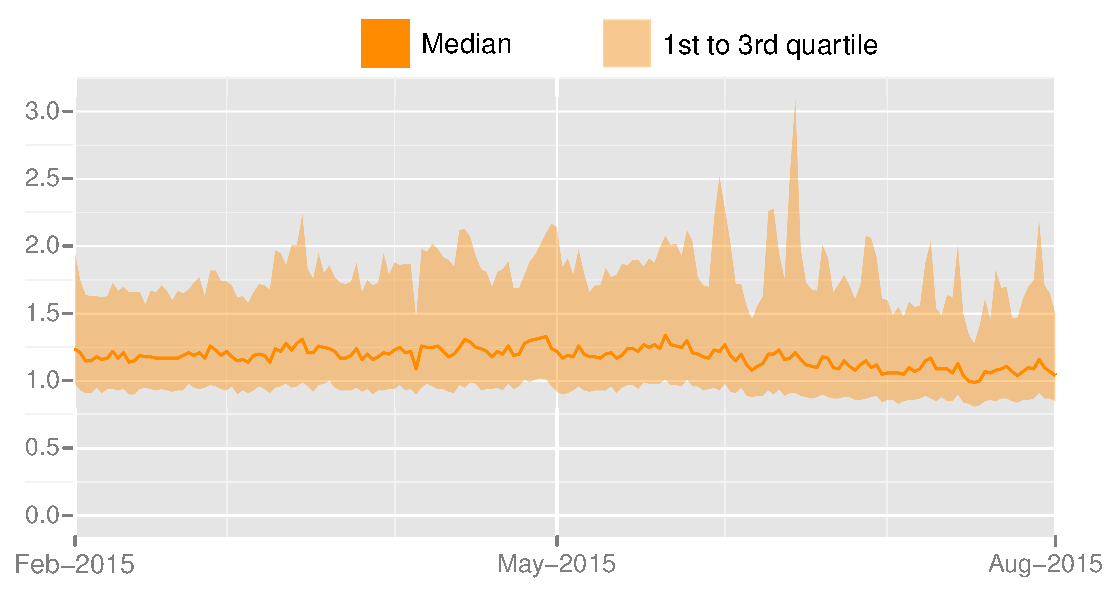
\includegraphics[width=\linewidth]{../assets/images/torperf_50kb_2015-02_2015-08.eps}
	\caption{The average performance to download 50 KB files over Tor circuits, as measured by Tor bandwidth authorities. The first and third quartiles are shown with the median time shown in orange\cite{TorMetrics}.}
	\label{fig:latencyGraph}
\end{figure}

This network latency is supplemental to the time to verify the Record and Merkle subtree. We avoid additional latency costs by implementing a client-side cache in order to allow subsequent queries to be resolved locally. We also reduce the expense of circuit construction by building the circuit on startup.

\section{Conclusions and Future Work}

We have presented the Onion Name System (OnioNS), a distributed, secure, and usable alternative DNS that maps globally-unique and meaningful .tor domains to .onion hidden service addresses, and achieve all three properties of Zooko's Triangle. We enable any hidden service operator to anonymously claim a human-readable name for their server and clients to query the system in privacy-enhanced manner. We introduce a distributed self-healing blockchain-based database and mechanisms that let clients authenticate and verify denial-of-existence claims. Additionally, we utilize the existing and semi-trusted infrastructure of Tor, which significantly narrows our threat model to already well-understood attack surfaces and allows our system to be integrated into Tor with minimal effort. Our reference implementation demonstrates high usability and shows that OnioNS successfully addresses the major usability issue that has been with Tor hidden services since their introduction in 2002.

In future work we will expand our implementation and pursuit integrating it into Tor. OnioNS requires a few changes to Tor, namely a new .tor pseudo-TLD and Ed25519 router keys, but we introduce no changes to Tor's hidden service protocol. Should Tor's developers introduce changes to the hidden service protocol, OnioNS can become forwards-compatible with a few changes. Additionally, our implementation currently only supports ASCII characters in domain names, so in future work we will explore implementing Punycode to provide support for international character sets. Unlike the Internet DNS, we will disallow digits zero and one (similar to base32 encoding) in order to reduce the threat of phishing attacks from spoofed domains with indistinguishable characters.

We will also explore the possibilities of hosting the OnioNS servers as hidden services. The Tor protocol provides defences against several network-level attacks and when combined with end-to-end authentication this approach may prove beneficial to our system.

\section*{Acknowledgements}

We would like to thank Roger Dingledine, George Kadianakis, Yawning Angel, and Nick Mathewson for their support, commentary, and assistance with Tor technical support.

%, a password-based key derivation function which is notable for its large memory and CPU requirements during its operation. The scrypt function provides significantly greater resistance to custom hardware attacks and massively parallel computation primarily due to its memory requirements. This limits attackers to the same software implementation and asymptotic cost as legitimate users\cite{percival2009stronger}\cite{percival2012scrypt}. We choose scrypt because of these advantages over other key derivation functions such as SHA-256 or PBKDF2. For these reasons scrypt is also common for proof-of-work purposes in some cryptocurrencies such as Litecoin.

% ----------------------------------------------------------------------------------------

% An example of a floating figure using the graphicx package.
% Note that \label must occur AFTER (or within) \caption.
% For figures, \caption should occur after the \includegraphics.
% Note that IEEEtran v1.7 and later has special internal code that
% is designed to preserve the operation of \label within \caption
% even when the captionsoff option is in effect. However, because
% of issues like this, it may be the safest practice to put all your
% \label just after \caption rather than within \caption{}.
%
% Reminder: the "draftcls" or "draftclsnofoot", not "draft", class
% option should be used if it is desired that the figures are to be
% displayed while in draft mode.
%
%\begin{figure}[!t]
%\centering
%\includegraphics[width=2.5in]{myfigure}
% where an .eps filename suffix will be assumed under latex, 
% and a .pdf suffix will be assumed for pdflatex; or what has been declared
% via \DeclareGraphicsExtensions.
%\caption{Simulation Results}
%\label{fig_sim}
%\end{figure}

% Note that IEEE typically puts floats only at the top, even when this
% results in a large percentage of a column being occupied by floats.

% ----------------------------------------------------------------------------------------

% An example of a double column floating figure using two subfigures.
% (The subfig.sty package must be loaded for this to work.)
% The subfigure \label commands are set within each subfloat command, the
% \label for the overall figure must come after \caption.
% \hfil must be used as a separator to get equal spacing.
% The subfigure.sty package works much the same way, except \subfigure is
% used instead of \subfloat.
%
%\begin{figure*}[!t]
%\centerline{\subfloat[Case I]\includegraphics[width=2.5in]{subfigcase1}%
%\label{fig_first_case}}
%\hfil
%\subfloat[Case II]{\includegraphics[width=2.5in]{subfigcase2}%
%\label{fig_second_case}}}
%\caption{Simulation results}
%\label{fig_sim}
%\end{figure*}
%
% Note that often IEEE papers with subfigures do not employ subfigure
% captions (using the optional argument to \subfloat), but instead will
% reference/describe all of them (a), (b), etc., within the main caption.

% ----------------------------------------------------------------------------------------

% An example of a floating table. Note that, for IEEE style tables, the 
% \caption command should come BEFORE the table. Table text will default to
% \footnotesize as IEEE normally uses this smaller font for tables.
% The \label must come after \caption as always.
%
%\begin{table}[!t]
%% increase table row spacing, adjust to taste
%\renewcommand{\arraystretch}{1.3}
% if using array.sty, it might be a good idea to tweak the value of
% \extrarowheight as needed to properly center the text within the cells
%\caption{An Example of a Table}
%\label{table_example}
%\centering
%% Some packages, such as MDW tools, offer better commands for making tables
%% than the plain LaTeX2e tabular which is used here.
%\begin{tabular}{|c||c|}
%\hline
%One & Two\\
%\hline
%Three & Four\\
%\hline
%\end{tabular}
%\end{table}

% ----------------------------------------------------------------------------------------

% Note that IEEE does not put floats in the very first column - or typically
% anywhere on the first page for that matter. Also, in-text middle ("here")
% positioning is not used. Most IEEE journals/conferences use top floats
% exclusively. Note that, LaTeX2e, unlike IEEE journals/conferences, places
% footnotes above bottom floats. This can be corrected via the \fnbelowfloat
% command of the stfloats package.

% conference papers do not normally have an appendix

% ----------------------------------------------------------------------------------------

% trigger a \newpage just before the given reference
% number - used to balance the columns on the last page
% adjust value as needed - may need to be readjusted if
% the document is modified later
%\IEEEtriggeratref{8}
% The "triggered" command can be changed if desired:
%\IEEEtriggercmd{\enlargethispage{-5in}}

% references section can use a bibliography generated by BibTeX as a .bbl file
% BibTeX documentation can be easily obtained at:
% http://www.ctan.org/tex-archive/biblio/bibtex/contrib/doc/
% The IEEEtran BibTeX style support page is at:
% http://www.michaelshell.org/tex/ieeetran/bibtex/
%\bibliographystyle{IEEEtranS}
% argument is your BibTeX string definitions and bibliography database(s)
%\bibliography{IEEEabrv,../bib/paper}
%
% <OR> manually copy in the resultant .bbl file
% set second argument of \begin to the number of references
% (used to reserve space for the reference number labels box)
%\begin{thebibliography}{1}
%
%\bibitem{IEEEhowto:kopka}
%H.~Kopka and P.~W. Daly, \emph{A Guide to \LaTeX}, 3rd~ed.\hskip 1em plus
%  0.5em minus 0.4em\relax Harlow, England: Addison-Wesley, 1999.
%
%\end{thebibliography}

\bibliographystyle{abbrv}
\bibliography{citations}

% that's all folks
\end{document}
